\def\thelstlisting{}

%不需要区分奇偶页的请使用下面一行
\documentclass[a4paper,AutoFakeBold,oneside,12pt]{book}
%需要区分奇偶页的(即每一章第一页一定在奇数页上)请使用下面一行
%\documentclass[a4paper,AutoFakeBold,openright,12pt]{book}
\usepackage{BUPTthesisbachelor}
\usepackage{setspace}

%\lstdefinestyle{sharpc}{language=[Sharp]C, frame=lrtb, rulecolor=\color{blue!80!black}}


%%%%%%%%%%%%%%%%%%%%%%%%% Begin Documents %%%%%%%%%%%%%%%%%%%%%%%%%%
\begin{document}

% 封面
\blankmatter

\includepdf[pages=-]{docs/cover.pdf}

% 任务书
% \blankmatter
% 
\includepdf[pages=-]{docs/task.pdf}

% 成绩评定表
% \blankmatter
% 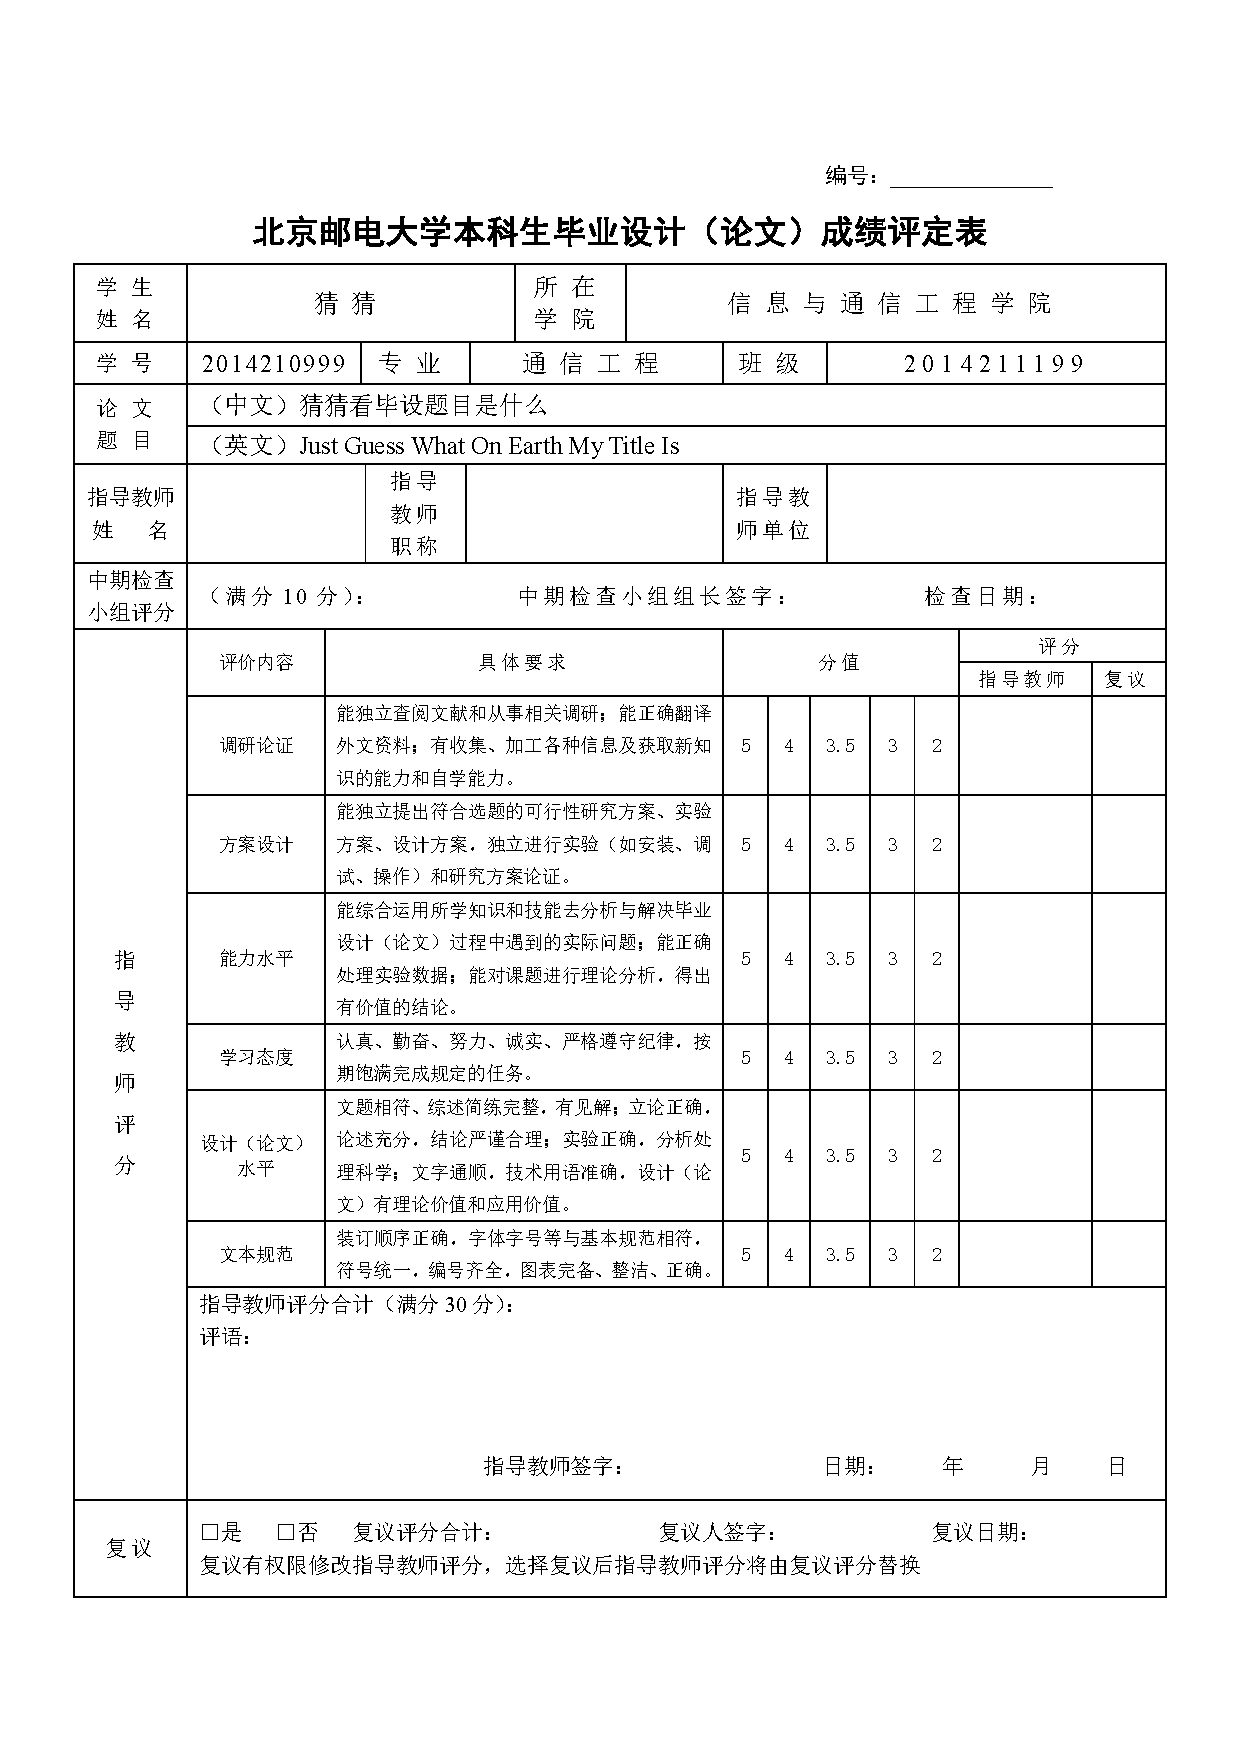
\includepdf[pages=-]{docs/scoreTable.pdf}

% 诚信声明
% \blankmatter
% 
\includepdf[pages=-]{docs/statement.pdf}

%%%%%%%%%%%%%%%%%%%%%%%%%%%%%%%%%%%%%%%%%%%%%%%%%%%%%%%%%%%%%%%%%%%%
%                                                                  %
%   Copyright (c) 2010 - 2011 Caspar Zhang <casparant@gmail.com>   %
%                                                                  %
%   This copyrighted material is made available to anyone wishing  %
%   to use, modify, copy, or redistribute it subject to the terms  %
%   and conditions of the GNU General Public License version 2.    %
%                                                                  %
%   This program is distributed in the hope that it will be        %
%   useful, but WITHOUT ANY WARRANTY; without even the implied     %
%   warranty of MERCHANTABILITY or FITNESS FOR A PARTICULAR        %
%   PURPOSE. See the GNU General Public License for more details.  %
%                                                                  %
%   You should have received a copy of the GNU General Public      %
%   License along with this program; if not, write to the Free     %
%   Software Foundation, Inc., 51 Franklin Street, Fifth Floor,    %
%   Boston, MA 02110-1301, USA.                                    %
%                                                                  %
%%%%%%%%%%%%%%%%%%%%%%%%%%%%%%%%%%%%%%%%%%%%%%%%%%%%%%%%%%%%%%%%%%%%

% 你只需要修改下面几行就可以完成大部分内容的填写,
% 这要求你具有一定的LaTeX基础,但是如果你足够聪明,
% 不具有LaTeX基础也可以完成。

% 论文中文题目
\def\thesistitle{社猜猜看这个毕设题目是什么}

% 论文英文题目
%提示:英文摘要页的标题注意格式要求。
\def\thesistitleen{HAVE A TRY TO GUESS WHAT THE TITLE IS}

% Thank Words
\def\thankwords{

此处请写致谢的内容。

它可以有多段。
}
    % Main items
% %%%%%%%%%%%%%%%%%%%%%%%%%%%%%%%%%%%%%%%%%%%%%%%%%%%%%%%%%%%%%%%%%%%%
%                                                                  %
%   Copyright (c) 2010 - 2011 Caspar Zhang <casparant@gmail.com>   %
%                                                                  %
%   This copyrighted material is made available to anyone wishing  %
%   to use, modify, copy, or redistribute it subject to the terms  %
%   and conditions of the GNU General Public License version 2.    %
%                                                                  %
%   This program is distributed in the hope that it will be        %
%   useful, but WITHOUT ANY WARRANTY; without even the implied     %
%   warranty of MERCHANTABILITY or FITNESS FOR A PARTICULAR        %
%   PURPOSE. See the GNU General Public License for more details.  %
%                                                                  %
%   You should have received a copy of the GNU General Public      %
%   License along with this program; if not, write to the Free     %
%   Software Foundation, Inc., 51 Franklin Street, Fifth Floor,    %
%   Boston, MA 02110-1301, USA.                                    %
%                                                                  %
%%%%%%%%%%%%%%%%%%%%%%%%%%%%%%%%%%%%%%%%%%%%%%%%%%%%%%%%%%%%%%%%%%%%

% 你只需要修改下面内容就可以完成中英文摘要,
% 这要求你具有一定的LaTeX基础,但是还是那句话,
% 如果你足够聪明,不具有LaTeX基础也可以完成。

% 中文摘要
\def\abstractzh{
%从这里开始写你的摘要,分段需要空一行。
这是中文摘要的部分。

它可以拥有多段。
这是中文摘要的部分。

它可以拥有多段。

如果你写的太长,甚至可以到第二页。
%摘要结束
}

% 中文关键字 
% TODO: 改成可变长度的
\def\abszhkeyone{北京邮电大学}
\def\abszhkeytwo{本科生}
\def\abszhkeythree{毕业设计}
\def\abszhkeyfour{模板}
\def\abszhkeyfive{示例}

% ABSTRACT
\def\abstracten{
%Your abstract here, to make a new paragraph, give an extra blank line please.
This is ABSTRACT.

You can write more than one paragraph here.

If your abstract is too long, it will take up more pages. 
%Abstract done
}

% Key Words 
% TODO: 改成可变长度的
\def\absenkeyone{BUPT}
\def\absenkeytwo{undergraduate}
\def\absenkeythree{thesis}
\def\absenkeyfour{template}
\def\absenkeyfive{example}


  % Abstract
\frontmatter\tableofcontents % Content
\fancypagestyle{plain}{\pagestyle{frontmatter}}

% 正文
\newpage\mainmatter
\fancypagestyle{plain}{\pagestyle{mainmatter}}
%\let\cleardoublepagebak=\cleardoublepage
%\let\cleardoublepage\relax % Make new chapter stay on old page

%%%%%%%%%%%%%%%%%%%%%%%%%%%%% Main Area %%%%%%%%%%%%%%%%%%%%%%%%%%%%
\chapter{背景知识}

\section{VOIP技术}
\subsection{VoIP简介}
互联网协议语音(也称为IP语音,VoIP或IP电话)是一种通过因特网协议(IP)网络传送语音通信和多媒体会话的方法和技术组。术语网络电话,宽带电话和宽带电话服务具体指的是通过公共互联网而不是通过公共交换电话网(PSTN)提供通信服务(语音,传真,SMS,语音消息)。

VoIP(Voice over Internet Protocol)简而言之就是将模拟信号(Voice)数字化,以数据封包(Data Packet)的形式在IP网络(IP Network)上做实时传递。VoIP最大的优势是能广泛地采用Internet和全球IP互连的环境,提供比传统业务更多、更好的服务。VoIP可以在IP网络上便宜的传送语音、传真、视频、和数据等业务,如统一消息业务、虚拟电话、虚拟语音/传真邮箱、查号业务、Internet呼叫中心、Internet呼叫管理、电话视频会议、电子商务、传真存储转发和各种信息的存储转发等。

\subsection{VoIP原理}
发起VoIP电话呼叫所涉及的步骤和原理类似于传统的数字电话,涉及信号,信道设置,模拟语音信号的数字化和编码。数字信息不是通过电路交换网络传输,而是打包,并且通过分组交换网络作为IP分组进行传输。它们使用特殊的媒体传输协议传输媒体流,该协议使用音频编解码器和视频编解码器对音频和视频进行编码。存在各种编解码器,其基于应用要求和网络带宽来优化媒体流;一些实现依赖于窄带和压缩语音,而其他实现则支持高保真立体声编解码器。一些流行的编解码器包括μ-law和A-law版本的G.711,G.722,一种称为iLBC的开源语音编解码器,一种仅使用8 kbit / s的编解码器,称为G.729,以及许多其他编解码器。

早期的IP语音服务提供商提供了商业模型和技术解决方案,它们反映了传统电话网络的架构。第二代提供商,如Skype,为私人用户群建立了封闭式网络,提供免费通话和便利的好处,同时可能为访问其他通信网络(如PSTN)收费。这限制了用户混合搭配第三方硬件和软件的自由。第三代提供商(如Google Talk)采用了联邦VoIP的概念,这与传统网络的体系结构不同。当用户希望拨打电话时,这些解决方案通常允许互联网上任何两个域上的用户之间的动态互连。

除VoIP电话外,VoIP还可用于许多个人计算机和其他互联网接入设备。可以通过移动数据或Wi-Fi发送呼叫和短信。VoIP允许使用单一统一通信系统整合现代通信技术(包括电话,智能电话,语音和视频会议,电子邮件和存在检测)。

\subsection{VoIP关键技术}
\subsubsection{常用协议简介}
已经使用基于开放标准的专有协议和协议以各种方式实现了IP语音。这些协议可以由VoIP电话,专用软件,移动应用程序使用或集成到网页中。VoIP协议包括:

\begin{itemize}
\item \textbf{会话发起协议(SIP)},由IETF开发的连接管理协议
\item \textbf{H.323},是第一个广泛实施的VoIP呼叫信令和控制协议之一。自从开发更新,更简单的协议(如MGCP和SIP)以来,H.323部署越来越局限于承载现有的长途网络流量。[需要引证]
\item \textbf{媒体网关控制协议(MGCP)},媒体网关的连接管理
\item \textbf{H.248},跨越融合互联网络的媒体网关的控制协议,包括传统的公共交换电话网(PSTN)和现代分组网络
\item \textbf{实时传输协议(RTP)},用于实时音频和视频数据的传输协议
\item \textbf{实时传输控制协议(RTCP)},用于RTP的姐妹协议,提供流统计和状态信息
\item \textbf{安全实时传输协议(SRTP)},RTP的加密版本
\item \textbf{会话描述协议(SDP)},主要由SIP用于描述VoIP连接的文件格式
\item \textbf{Inter-Asterisk eXchange(IAX)},VoIP服务器之间使用的协议
\item \textbf{可扩展消息和状态协议(XMPP)},即时消息,状态信息和联系人列表维护
\item \textbf{Jingle},为XMPP添加了点对点会话控制
\item \textbf{Skype协议},基于点对点架构的专有Internet电话协议套件。
\end{itemize}

\subsubsection{其它关键技术}

\begin{itemize}
\item \textbf{媒体编码技术},主要包括的G.711、G.723.1和G.729等多媒体压缩编码技术。
\item \textbf{媒体实时传输技术},主要采用实时传输协议RTP。
\item \textbf{业务质量保障技术},采用资源预留协议RSVP等。
\item \textbf{网络传输技术},主要是TCP和UDP。
\end{itemize}

\section{SIP技术}
\subsection{SIP简介}
会话发起协议(SIP)是一种信令协议,用于发起,维护和终止包括语音,视频和消息传递应用的实时会话。SIP用于在用于语音和视频呼叫的因特网电话的应用中,在专用IP电话系统中,在因特网协议(IP)网络上的即时消息传送以及通过LTE的移动电话呼叫(VoLTE)中的信令和控制多媒体通信会话。

该协议定义了交换的消息的特定格式以及参与者合作的通信顺序。 SIP是一种基于文本的协议,包含超文本传输协议(HTTP)和简单邮件传输协议(SMTP)的许多元素。使用SIP建立的呼叫可以包括多个媒体流,但是在SIP消息中作为有效载荷交换数据的应用(例如文本消息)不需要单独的流。

SIP与指定和携带会话媒体的其他几种协议一起使用。最常见的是,媒体类型和参数协商以及媒体设置使用会话描述协议(SDP)来执行,该协议作为SIP消息中的有效载荷来承载。 SIP被设计为独立于底层传输层协议,并且可以与用户数据报协议(UDP),传输控制协议(TCP)和流控制传输协议(SCTP)一起使用。对于通过不安全网络链路的SIP消息的安全传输,可以使用传输层安全性(TLS)来加密协议。对于媒体流(语音,视频)的传输,SIP消息中携带的SDP有效载荷通常采用实时传输协议(RTP)或安全实时传输协议(SRTP)。

\subsection{SIP结构}
\subsubsection{协议操作}

%图片宽度设置为文本宽度的75%,可以调整为合适的比例
\buptfigure[width=0.7\textwidth]{pictures/fig1.png}{SIP用户代理向SIP注册器注册并进行身份验证}{fig1}

SIP仅涉及媒体通信会话的信令操作,主要用于建立和终止语音或视频呼叫。 SIP可用于建立双方(单播)或多方(多播)会话。它还允许修改现有的呼叫。修改可涉及更改地址或端口,邀请更多参与者,以及添加或删除媒体流。 SIP还在消息传递应用程序中找到了应用程序,例如即时消息传递,事件订阅和通知。

SIP与其他几种协议协同工作,这些协议指定媒体格式和编码,并在呼叫建立后携带媒体。对于呼叫建立,SIP消息的主体包含会话描述协议(SDP)数据单元,其指定媒体格式,编解码器和媒体通信协议。语音和视频媒体流通常使用实时传输协议(RTP)或安全实时传输协议(SRTP)在终端之间传输。

SIP网络的每个资源(例如用户代理,呼叫路由器和语音邮箱)由统一资源标识符(URI)标识。 URI的语法遵循Web服务和电子邮件中也使用的通用标准语法。用于SIP的URI方案是sip,典型的SIP URI的格式为sip:username @ domainname或sip:username @ hostport,其中domainname需要DNS SRV记录来定位SIP域的服务器,而hostport可以是IP地址或者主机和端口的完全限定域名。如果需要安全传输,则使用方案啜饮。

SIP采用类似于HTTP请求/响应事务模型的设计元素。每个事务由一个客户端请求组成,该请求调用服务器上的特定方法或函数以及至少一个响应。 SIP重用HTTP的大多数头字段,编码规则和状态代码,提供可读的基于文本的格式。

SIP可以由若干传输层协议承载,包括传输控制协议(TCP),用户数据报协议(UDP)和流控制传输协议(SCTP)。SIP客户端通常在端口号5060或5061上使用TCP或UDP来获取到服务器和其他端点的SIP流量。端口5060通常用于非加密信令流量,而端口5061通常用于使用传输层安全性(TLS)加密的流量。

基于SIP的电话网络通常实现信号系统7(SS7)的呼叫处理功能,其中存在特殊的SIP协议扩展,尽管这两种协议本身是非常不同的。 SS7是一种集中式协议,其特点是复杂的中央网络架构和哑终端(传统电话手机)。 SIP是等效同伴的客户端 - 服务器协议。 SIP功能在通信端点中实现,而传统SS7架构仅在交换中心之间使用。

\buptfigure[width=0.7\textwidth]{pictures/fig2.png}{SIP用户代理向SIP注册器注册并进行身份验证}{fig2}

\subsubsection{网络元素}
使用会话发起协议进行通信的网络元素称为SIP用户代理。每个用户代理(UA)在请求服务功能时执行用户代理客户端(UAC)的功能,在响应请求时执行用户代理服务器(UAS)的功能。因此,任何两个SIP端点原则上可以在没有任何中间SIP基础设施的情况下操作。但是,出于网络操作原因,为了向用户提供公共服务以及为目录服务,SIP定义了几种特定类型的网络服务器元素。这些服务元素中的每一个还在用户代理客户端和服务器中实现的客户端 - 服务器模型内通信。

用户代理是发送或接收SIP消息并管理SIP会话的逻辑网络端点。用户代理具有客户端和服务器组件。用户代理客户端(UAC)发送SIP请求。用户代理服务器(UAS)接收请求并返回SIP响应。与修复客户端和服务器角色的其他网络协议不同,例如在HTTP中,其中Web浏览器仅充当客户端,而从不充当服务器,SIP要求两个对等体都实现这两种角色。 UAC和UAS的角色仅在SIP事务期间持续。

SIP电话是一种IP电话,它实现SIP用户代理的客户端和服务器功能,并提供电话的传统呼叫功能,如拨号,接听,拒绝,呼叫保持和呼叫转移。SIP电话可以实现为硬件设备或软电话。随着供应商越来越多地将SIP实施为标准电话平台,基于硬件和基于软件的SIP电话之间的区别是模糊的,并且SIP元件在许多具有IP功能的通信设备(例如智能电话)的基本固件功能中实现。

\buptfigure[width=0.7\textwidth]{pictures/fig3.png}{User1的UAC使用Invite Client Transaction发送初始INVITE(1)消息}{fig3}

示例:User1的UAC使用Invite Client Transaction发送初始INVITE(1)消息。 如果在定时器控制的等待时段之后没有接收到响应,则UAC可以选择终止事务或重新发送INVITE。 收到回复后,User1确信INVITE已可靠传送。 然后,User1的UAC必须确认响应。 在交付ACK(2)时,交易的双方都已完成。 在这种情况下,可能已经建立了一个对话框。

在SIP中,如在HTTP中,用户代理可以使用消息头字段(用户代理)来标识自己,该消息头字段包含软件,硬件或产品名称的文本描述。用户代理字段在请求消息中发送,这意味着接收SIP服务器可以评估此信息以执行特定于设备的配置或功能激活。 SIP网络元素的运营商有时会将此信息存储在客户帐户门户中,它可用于诊断SIP兼容性问题或显示服务状态。

代理服务器是具有UAC和UAS组件的网络服务器,其充当中间实体以便代表其他网络元件执行请求。代理服务器主要扮演路由的角色,这意味着它的工作是确保将请求发送到更靠近目标用户的另一个实体。代理对于实施策略也是有用的,例如用于确定是否允许用户进行呼叫。代理解释,并在必要时,在转发请求消息之前重写请求消息的特定部分。

SIP用户代理向SIP注册器注册并进行身份验证。注册商是提供位置服务的SIP端点。它接受REGISTER请求,记录用户代理的地址和其他参数。对于后续请求,它提供了在网络上定位可能的通信对等体的基本手段。位置服务将一个或多个IP地址链接到注册代理的SIP URI。多个用户代理可以注册相同的URI,结果是所有注册的用户代理都接收对URI的调用。

\subsection{SIP地址和命名规则}
SIP消息的地址信息是基于SIP通用资源定位标记(URL)定义的:

\buptfigure[width=0.7\textwidth]{pictures/fig4.png}{SIP消息的地址信息}{fig4}

\chapter{开源程序说明}
\section{PJSIP}
\subsection{PJSIP简介}
PJSIP是一个用C语言编写的免费开源多媒体通信库,实现了基于标准的协议,如SIP,SDP,RTP,STUN,TURN和ICE。 它将信令协议(SIP)与丰富的多媒体框架和NAT遍历功能结合到高级API中,该API可移植,适用于从桌面,嵌入式系统到移动手持设备的几乎任何类型的系统。\cite{webster_pjsip}

PJSIP既紧凑又功能丰富。 它支持音频,视频,状态和即时消息,并具有丰富的文档。 PJSIP非常便携。 在移动设备上,它抽象出系统相关的功能,并且在许多情况下能够利用设备的本机多媒体功能。

\subsection{PJSIP优点}

PJSIP试图为开发人员提供构建实时多媒体通信应用所需的一切。 PJSIP已经处理了实时多媒体应用的所有三个主要组件,即信令,媒体特征和NAT遍历。把这些留给我们,你可以专注于应用程序逻辑。

\begin{enumerate}
\item \textbf{完整和整合}

PJSIP试图为开发人员提供构建实时多媒体通信应用所需的一切。 PJSIP已经处理了实时多媒体应用的所有三个主要组件,即信令,媒体特征和NAT遍历。把这些留给我们,你可以专注于应用程序逻辑。
\item \textbf{非常便携}

编写您的应用程序一次,它将运行在任何类型的Windows,Windows Mobile / CE至WM 6,Mac OS X PPC和Intel,任何处理器类型的Linux,多种Unix系统,Nokia / Symbian 3rd和5th版本设备,iPhone,iPad和iPod上的Apple iOS,BlackBerry 10和Android(计划在v2.2中)。PJSIP也被用于嵌入式系统,人们报告在不同类型的处理器上成功使用嵌入式OS / RTOS,如uC-Linux,QNX和RTEMS。 PJSIP运行在20Mhz MIPS处理器设备上。
\item \textbf{紧凑,小而精悍}

语音呼叫应用程序使用较低级别的库从低至150KB开始,或使用较高级别的PJSUA-LIB API从几百KB开始,这两个API使用几百KB的堆使用。足迹当然会随着使用的功能而变化,但希望这给出了广泛的指示。
\item \textbf{完整的文档}

我们还努力编写文档。在API的参考文档之上,我们在(Trac)wiki站点上写了很多文章来帮助您进行开发。所有PJSIP文档都在Trac站点中编制索引。
\item \textbf{成熟}

PJSIP已经解决了许多现实问题,并且应用许多技巧来使事情发挥作用。
\item \textbf{专业开源}

最后但同样重要的是,PJSIP是开源软件(OSS)。开源已经使PJSIP能够被全球数千名开发人员使用,并且可能也被许多开发者仔细审查。寻找PJSIP开发人员变得越来越容易,作为开源软件,即使离开开发人员,PJSIP代码也永远不会消失。
\end{enumerate}

\subsection{PJSIP框架}
PJSIP包括以下几部分:

\begin{itemize}
\item PJSIP - Open Source SIP Stack[开源的SIP协议栈]
\item PJMEDIA - Open Source Media Stack[开源的媒体栈]
\item PJNATH - Open Source NAT Traversal Helper Library[开源的NAT-T辅助库]
\item PJLIB-UTIL - Auxiliary Library[辅助工具库]
\item PJLIB - Ultra Portable Base Framework Library[基础框架库]
\end{itemize}

PJMEDIA是一个为PJSIP建立一个完整特性SIP用户代理应用提供的补充库,这些应用包括:softphones/hardphones,gateways or B2BUA. 使用PJSIP与PJMEDIA一起开发的应用,其具备如下的特性:

\begin{itemize}
\item 高度的可移殖性,与PJSIP/PJLIB一起,PJMEDIA可运行在许多平台上,包括服务器、桌面、PDA系统,定制的硬件、PDA或移动电话。
\item 多种功能:会议桥接、多种编解码器、丢包隐蔽/ PLC,音频发生器,静音探测器,声学回声消除/ AEC,RFC2833,RTP / RTCP协议栈,speex/iLBC/GSM/G.711编解码器等 。
\item 高质量:PJMEDIA支持频率为16KHz、32Khz的编码和解码,事实上能支持任何音频采样率,可提供高质量的采样转换。 PJMEDIA也可以容忍一定量的网络或声音设备的不稳定和一些数据包丢失。
\item 很好的支持嵌入式/DSP:占用内存小,灵活性好。该媒体组件被设计成可替换成相应功能的硬件。
\end{itemize}

PJNATH是一个新的库,帮助应用程序进行NAT穿越。它实现了NAT穿越的最新规范:STUN、TURN和ICE。 PJNATH可以作为一个独立库,在您的软件中使用,也可以使用PJSUA- LIB库,该库很好的与PJSIP,PJMEDIA和PJNATH整合在一起,使用起来比较简单。 PJNATH有以下特点:

\begin{itemize}
\item STUNbis实现,实现符合RFC5389标准。既提供需要使用的STUN网络接口,又提供基于STUN但更高层次的框架,既TURN和ICE。
\item NAT类型检测,
根据RFC3489(STUN) ,在前端可以执行NAT类型检测。该检测方法不能对所有NAT类型进行穿越,但该信息可能仍然是有用,以便进行故障排除,已经被ICE整合,因此提供了该检测方式。
\item TURN实现,TURN是一个中继通信协议,通过使用中继,并结合ICE,提供了高效的最低代价的通信路径。PJNATH中TURN的实现,符合draft-ietf-behave-turn-14草案。ICE实现,ICE是一个发现两个端点之间的通信路径协议。PJNATH中ICE的实现符合draft-ietf-mmusic-ice-19.txt草案在未来,将实现更多的协议(如UPnP IGD和SOCKS5)。
\end{itemize}

PJLIB-UTIL是一个辅助库,为PJMEDIA和PJSIP提供支持。这个库中的一些功能/组件:占用内存小的XML解析,STUN客户端库,异步/缓存DNS解析,哈希/加密功能等 。占用内存小,高性能,高可移植性的抽象库和框架,被PJSIP和PJMEDIA使用。

PJLIB是PJLIB-UTIL、PJMEDIA和PJSIP唯一依赖的库,因为它提供了完整的抽象,不仅仅是操作系统依赖的属性,还包括LIBC的抽象,并提供了一些有用的数据结构。 PJLIB基础框架库提供的功能:

\begin{itemize}
\item 内存的处理、数据的存储;数据结构的(hash表、link表、二叉树、等);
\item caching和pool;缓冲池和内存池;
\item OS抽象;
\item 线程、互斥、临界区、锁对象、事件对象;
\item 定时器,$pj_str_t$字符串,操作系统级别的函数抽像,socket的抽象(tcp/udp) ,文件的读写,使用前的初始化,使用后的清理。
\end{itemize}

PJSIP库框架如下图\ref{fig5}:

\buptfigure[width=0.7\textwidth]{pictures/fig5.jpg}{PJSIP库框架结构图}{fig5}

\chapter{实验过程和结果}
\section{下载开源代码,学习官方文档}

\begin{enumerate}
\item 下载pjsip的源代码并阅读学习pjsip的编译说明。
\item 下载VS2015并熟悉编译环境。
\end{enumerate}

\section{编译开源工程文件}
\subsection{准备工作}
本次实验在VS2015的环境下运行编译。

\subsection{编译源程序}
打开源文件,并且右键pjsua,设置默认启动项目并编译,项目工程目录结构如图\ref{fig6}所示:

\buptfigure[width=0.7\textwidth]{pictures/fig6.png}{VS2015工程目录结构}{fig6}

\section{PJSIP进行通话}
\subsection{注册}

\begin{enumerate}
\item 运行PJSIP客户端文件,如下:

\buptfigure[width=0.7\textwidth]{pictures/fig7.png}{软件注册界面}{fig7}

\item 输入m,开始进行呼叫,然后输入IVR的SIP地址,命令为:sip:12345@10.105.242.72
\end{enumerate}

注册过程如下(注意:根据语音提示,注意每一步输入数据时,都要先输入*键,然后才能输入有效数据。具体操作步骤如下:):

\buptfigure[width=0.7\textwidth]{pictures/fig8.png}{软件注册过程}{fig8}

\subsection{验证组号和学号}
步骤如下:

\buptfigure[width=0.7\textwidth]{pictures/fig9.png}{验证组号和学号}{fig9}

\subsection{测试录音以及回放}
步骤与验证学号相似,不再说明

\section{Wireshark抓包分析}
\subsection{Wireshark准备工作}
打开程序后,需要选定抓取数据的网卡,这里只有一个本地连接,默认选择后,点击Start开始进行抓包。如果不进行过滤的话,会把所有数据包都抓到,这样数据量太多,不易分析。需要在Filter添加过滤条件sip,以便方便查看我们需要得到的数据包,这样就过滤掉非sip的数据包。
\subsection{Wireshark抓取并分析数据包}
做一个登录查询本组学号的的抓包实验,然后进行下列分析。
当完成操作后,抓取到相应的数据包如下图:

\buptfigure[width=0.7\textwidth]{pictures/fig10.png}{Wireshark抓取到的数据包}{fig10}

分析确认请求的数据包,能看到一些信息如下图:

\buptfigure[width=0.7\textwidth]{pictures/fig11.png}{Wireshark抓取到的数据包信息}{fig11}

继续分析:点击Wireshark菜单栏中的”Telephony”工具,选择“VoIP  Calls”工具,如下图:

\buptfigure[width=0.7\textwidth]{pictures/fig12.png}{Wireshark抓取到的数据包Telephony分析结果}{fig12}

然后,选中该sip的通讯过程,点击“Flow Sequence”按钮,便可以查看双方的通话过程:

\buptfigure[width=0.7\textwidth]{pictures/fig13.png}{通话过程}{fig13}

结果如下两图:

\begin{figure}[!htbp]
	\centering
	\subfloat[]{ %[]对齐方式,t为top,b为bottom,留空即可
\label{Fig:R1} % 子图1标签名
		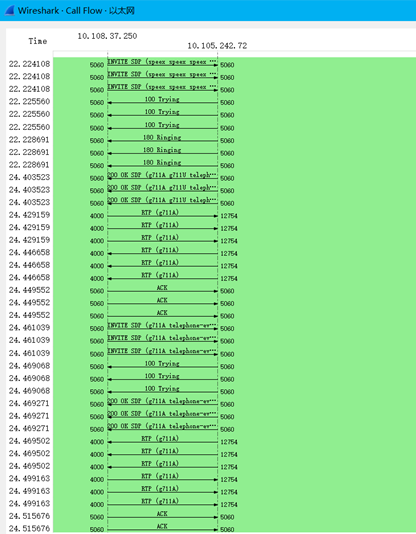
\includegraphics[width=0.45\textwidth]{pictures/fig14} %插入图片命令,格式为[配置]{图片路径}
	}
	\quad %空格
	\subfloat[]{
\label{Fig:R2} % 子图2标签名
		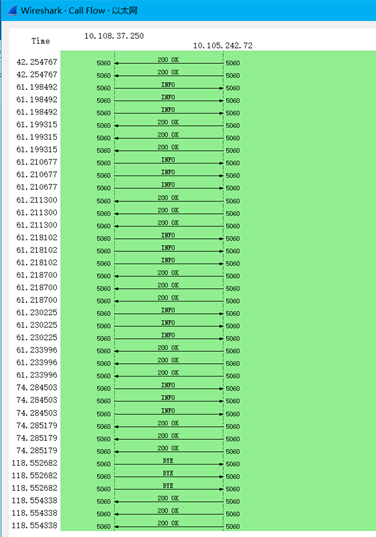
\includegraphics[width=0.45\textwidth]{pictures/fig15}
	}
	\caption{SIP通信过程:\protect\subref{Fig:R1}第一部分,\protect\subref{Fig:R2}第二部分} %注意须使用\protect\subref{}进行标号引用
	\label{Fig:RecAccuracy} % 整个组图的标签名
\end{figure}

上述是登录查询学号时的抓包实验,然后又进行了小组录音和回放等实验,数据包分析和上述大体相似,在此不一一截图描述了。

\section{问题及解决方法}
\subsection{输入超时}
在刚开始直接输入数字及$\sharp$号键时,会出现无法识别输入,应该在输入前先输入$\ast$号键再回车得到有效输入,如下图:

\buptfigure[width=0.7\textwidth]{pictures/fig16.png}{输入超时}{fig16}


% \chapter{基础模块示例}

% % 如果你的项目来源于科研项目,可以使用以下指令插入无编号脚注于正文第一页
% \blfootnote{本项目来源于科研项目“基于\LaTeX{}的本科毕业设计”,项目编号1124}

% \section{特殊文本类型}
% \subsection{脚注}
% 社交媒体是一种供用户创建在线社群来分享信息、观点、个人信息和其它内容(如视频)的电子化交流平台,社交网络服务(social network service, SNS)和微博客(microblogging)都属于社交媒体的范畴\cite{webster_social_media},国外较为知名的有Facebook\footnote{http://www.facebook.com/}、Instagram\footnote{https://www.instagram.com/}、Twitter\footnote{http://www.twitter.com/}、LinkedIn\footnote{http://www.linkedin.com/}等,国内较为知名的有新浪微博\footnote{http://www.weibo.com/}。

% 在社交媒体的强覆盖下,新闻信息的传播渠道也悄然了发生变化。\cite{false_news_spread_2018}

% \subsection{定义、定理与引理等}
% \begin{definition}
% 这是一条我也不知道在说什么的定义,反正我就是写在这里做个样子罢了,也没人会仔细读。\cite{周兴2017基于深度学习的谣言检测及模式挖掘}
% \end{definition}

% \begin{theorem}
% 这是一条我也不知道在说什么的定理,反正我就是写在这里做个样子罢了,也没人会仔细读。
% \end{theorem}

% \begin{axiom}
% 这是一条我也不知道在说什么的公理,反正我就是写在这里做个样子罢了,也没人会仔细读。
% \end{axiom}

% \begin{lemma}
% 这是一条我也不知道在说什么的引理,反正我就是写在这里做个样子罢了,也没人会仔细读。
% \end{lemma}

% \begin{proposition}
% 这是一条我也不知道在说什么的命题,反正我就是写在这里做个样子罢了,也没人会仔细读。
% \end{proposition}

% \begin{corollary}
% 这是一条我也不知道在说什么的推论,反正我就是写在这里做个样子罢了,也没人会仔细读。
% \end{corollary}

% \subsection{中英文文献、学位论文引用}
% 根据美国皮尤研究中心的2017年9月发布的调查结果\cite{pew_news_use_2017},67\%的美国民众会从社交媒体上获取新闻信息,其中高使用频率用户占20\%。在国内,中国互联网信息中心《2016年中国互联网新闻市场研究报告》\cite{internet_news_2016}也显示,社交媒体已逐渐成为新闻获取、评论、转发、跳转的重要渠道,在2016年下半年,曾经通过社交媒体获取过新闻资讯的用户比例高达90.7\%,在微信、微博等社交媒体参与新闻评论的比例分别为62.8\%和50.2\%。社交媒体正在成为网络上热门事件生成并发酵的源头,在形成传播影响力后带动传统媒体跟进报道,最终形成更大规模的舆论浪潮。\cite{Yang2012Automatic}

% 在国内,新浪微博由于其发布方便、传播迅速、受众广泛且总量大的特点,成为了虚假信息传播的重灾区:《中国新媒体发展报告(2013)》\cite{唐绪军2013中国新媒体发展报告}显示,2012年的100件微博热点舆情案例中,有超过1/3出现谣言;《中国新媒体发展报告(2015)》\cite{唐绪军2015中国新媒体发展报告}对2014年传播较广、比较典型的92条假新闻进行了多维度分析,发现有59\%的虚假新闻首发于新浪微博。

% 此等信息的传播严重损害了有关公众人物的名誉权,降低了社交媒体服务商的商业美誉度,扰乱了网络空间秩序,冲击着网民的认知,极易对民众造成误导,带来诸多麻烦和经济损失,甚至会导致社会秩序的混乱。针对社交媒体谣言采取行动成为了有关部门、服务提供商和广大民众的共同选择。\cite{周兴2017基于深度学习的谣言检测及模式挖掘}

% \section{图表及其引用}
% 此处引用了简单的表\ref{crowdwisdom_TMP}。

% 请注意,\LaTeX{}的图表排版规则决定了图表\textbf{不一定会乖乖呆在你插入的地方},这是为了避免Word中由于图片尺寸不匹配在页面下部出现的的空白,所以请不要使用“下图”“下表”作为指向文字,应使用“图1-1所示”这样的表述。

% \begin{bupttable}{基于浏览者行为的特征}{crowdwisdom_TMP}

%     \begin{tabular}{l|l|l}
% 		\hline \textbf{特征} & \textbf{描述} & \textbf{形式与理论范围}\\
% 		\hline 点赞量 & 微博的点赞数量 & 数值,$\mathbb{N}$ \\
% 		\hline 评论量 & 微博的评论数量 & 数值,$\mathbb{N}$ \\
% 		\hline 转发量 & 微博的转发数量 & 数值,$\mathbb{N}$ \\
% 		\hline
%     \end{tabular}
% \end{bupttable}

% 此处引用了复杂的表\ref{complexcrowdwisdom_TMP}。


% \begin{bupttable}{基于浏览者行为的复杂特征}{complexcrowdwisdom_TMP}
%     \begin{tabular}{l|l|l|l}
%         \hline
%         \multicolumn{1}{c|}{\multirow{2}{*}{\textbf{类别}}} & \multicolumn{1}{c|}{\multirow{2}{*}{\textbf{特征}}} & \multicolumn{2}{c}{\textbf{不知道叫什么的表头}} \\
%         \cline{3-4}
%         & & \multicolumn{1}{c|}{\textbf{描述}} & \multicolumn{1}{c}{\textbf{形式与理论范围}} \\
%         \hline
%         \multirow{3}{*}{正常互动} & 点赞量 & 微博的点赞数量 & 数值,$\mathbb{N}$ \\
%         \cline{2-4}
%         & 评论量 & 微博的评论数量 & 数值,$\mathbb{N}$ \\
%         \cline{2-4}
%         & 转发量 & 微博的转发数量 & 数值,$\mathbb{N}$ \\
%         \hline
%         非正常互动 & 羡慕量 & 微博的羡慕数量 & 数值,$\mathbb{N}$ \\
%         \hline
%     \end{tabular}
% \end{bupttable}

% 此处展示了更专业的表\ref{tab:abbr_table},一个好的表格没有竖线。
% % 请注意1)tabularx环境对多行文本的处理;2)booktabs宏包中支持的更粗的顶端和底端表格边界线,边界线与文本间更大的间距。
% \begin{bupttable}{红警2名词解释}{tab:abbr_table}
%     \begin{tabularx}{\textwidth}{llX}
%         \toprule
%         \textbf{术语类别} & \textbf{缩略语} & \textbf{解释} \\ \midrule
%         & 兵营 & 兵营(Barracks),《命令与征服\ 红色警戒2:尤里的复仇》游戏中的一种生产建筑,用以生产步兵单位 \\ \cmidrule(l){2-3}
%         & 建造场 & 建造场(Construction Yard),《命令与征服\ 红色警戒2:尤里的复仇》游戏中的一种基础建筑,用以支持其他建筑的建造 \\ \cmidrule(l){2-3}
%         & 矿厂 & 矿石精炼厂(Ore Refinery),《命令与征服\ 红色警戒2:尤里的复仇》游戏中的一种资源建筑,用以将矿车采集的矿石转化为游戏资金 \\ \cmidrule(l){2-3}
%         游戏 & 空指 & 空指部(Airforce Command Headquarters),《命令与征服\ 红色警戒2:尤里的复仇》游戏中的一种资源建筑,用以提供雷达功能和T2科技及生产部分空军单位 \\ \cmidrule(l){2-3}
%         & 相机 & 游戏术语,特指游戏内的观察区域和视角 \\ \cmidrule(l){2-3}
%         & 重工 & 战车工厂(War Factory),《命令与征服\ 红色警戒2:尤里的复仇》游戏中的一种生产建筑,用以生产载具单位 \\ \cmidrule(l){2-3}
%         & 战争迷雾 & 游戏术语,《命令与征服\ 红色警戒2:尤里的复仇》中指黑色的未探索区域 \\ \bottomrule
%     \end{tabularx}
% \end{bupttable}

% 此处引用了一张图。图\ref{autoencoder_TMP}表示的是一个由含有4个神经元的输入层、含有3个神经元的隐藏层和含有4个神经元的输出层组成的自编码器,$+1$代表偏置项。

% %图片宽度设置为文本宽度的75%,可以调整为合适的比例
% \buptfigure[width=0.7\textwidth]{pictures/autoencoder}{自编码器结构}{autoencoder_TMP}

% %组图示例,已按照指导手册要求设计,由于子图数量不同,无法压缩成\buptfigure那样,大家对照示例即可
% \begin{figure}[!htbp]
%     \centering
%     \subfloat[]{ %[]对齐方式,t为top,b为bottom,留空即可
% 	\label{Fig:R1} % 子图1标签名
%     	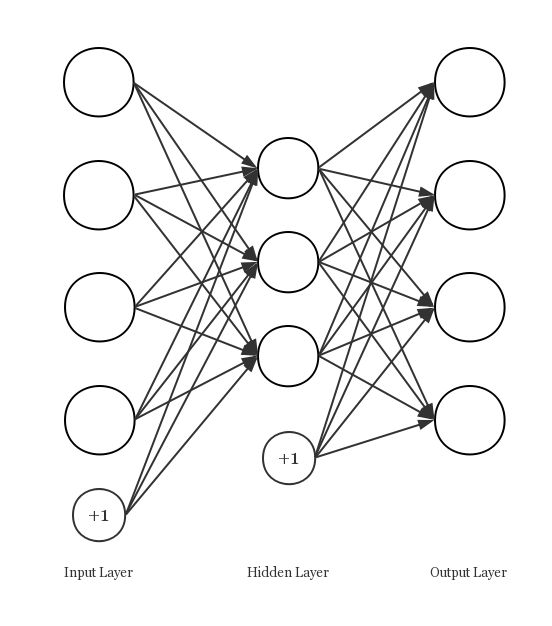
\includegraphics[width=0.45\textwidth]{pictures/autoencoder} %插入图片命令,格式为[配置]{图片路径}
%     }
%     \quad %空格
%     \subfloat[]{
% 	\label{Fig:R2} % 子图2标签名
%     	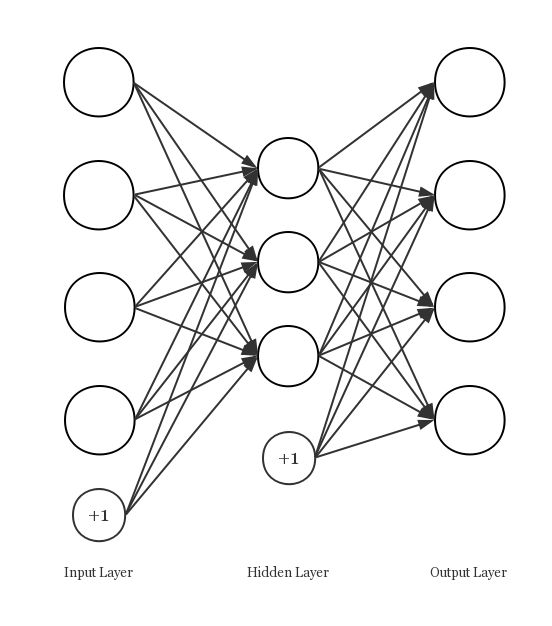
\includegraphics[width=0.45\textwidth]{pictures/autoencoder}
%     }
%     \caption{这是两个自编码器结构,我就是排一下子图的效果:\protect\subref{Fig:R1}左边的自编码器,\protect\subref{Fig:R2}右边的自编码器} %注意须使用\protect\subref{}进行标号引用
%     \label{Fig:RecAccuracy} % 整个组图的标签名
% \end{figure}

% \section{公式与算法表示}

% \subsection{例子:基于主成分分析}

% \subsubsection{主成分分析算法}

% 下面对主成分分析进行介绍。

% 主成分分析是一种简单的机器学习算法,其功能可以从两方面解释:一方面可以认为它提供了一种压缩数据的方式,另一方面也可以认为它是一种学习数据表示的无监督学习算法。\cite{Goodfellow2016DeepLearning}
% 通过PCA,我们可以得到一个恰当的超平面及一个投影矩阵,通过投影矩阵,样本点将被投影在这一超平面上,且满足最大可分性(投影后样本点的方差最大化),直观上讲,也就是能尽可能分开。

% 对中心化后的样本点集$\bm{X}=\{\bm{x}_1,\bm{x}_2,\ldots,\bm{x}_i,\ldots,\bm{x}_m\}$(有$\sum_{i=1}^{m}\bm{x}_i = 0$),考虑将其最大可分地投影到新坐标系\ $\bm{W}= \{\bm{w}_1,\bm{w}_2,\ldots,\bm{w}_i,\ldots,\bm{w}_d\} $,其中$\bm{w}_i$是标准正交基向量,满足$\|\bm{w}_i\|_2 = 1$, $\bm{w}_i^T\bm{w}_j = 0$($i \not= j$)。假设我们需要$d^\prime$($d^\prime < d$)个主成分,那么样本点$\bm{x}_i$在低维坐标系中的投影是$\bm{z}_i = (z_{i1};z_{i2};\ldots;z_{id^\prime})$,其中$z_{ij} = \bm{w}_j^\mathrm{T}\bm{x}_i$,是$\bm{x}_i$在低维坐标系下第$j$维的坐标。
% 对整个样本集,投影后样本点的方差是
% \begin{equation}
% \begin{aligned}
%     & \frac{1}{m}\sum_{i=1}^m \bm{z}_i^\mathrm{T}\bm{z}_i \\
% = & \frac{1}{m}\sum_{i=1}^m (\bm{x}_i^\mathrm{T}\bm{W})^\mathrm{T}(\bm{x}_i^\mathrm{T}\bm{W}) \\
% = & \frac{1}{m}\sum_{i=1}^m \bm{W}^\mathrm{T}\bm{x}_i\bm{x}_i^\mathrm{T}\bm{W} \\
% = & \frac{1}{m} \bm{W}^\mathrm{T}\bm{X}\bm{X}^\mathrm{T}\bm{W} \\
% \end{aligned}
% \end{equation}

% 由于我们知道新坐标系$\bm{W}$的列向量是标准正交基向量,且样本点集$\bm{X}$已经过中心化,则PCA的优化目标可以写为
% \begin{equation}
% \label{PCA_goal_TMP}
% \begin{aligned}
% & \max_{\substack{\bm{W}}}  &  tr(\bm{W}^\mathrm{T}\bm{X}\bm{X}^ \mathrm{T}\bm{W}) \\
% & \operatorname{ s.t. }  &  \bm{W}^\mathrm{T}\bm{W} = \bm{I} \\
% \end{aligned}
% \end{equation}

% 由于$\bm{X}\bm{X}^ \mathrm{ T }$是协方差矩阵,那么只需对它做特征值分解,即
% \begin{equation}
% \label{PCA_eigenvalue}
% \bm{X}^ \mathrm{ T }\bm{X} = \bm{W}\bm{\Lambda}\bm{W}^ \mathrm{ T } \\
% \end{equation}
% 其中$\bm{\Lambda}=diag(\bm{\lambda})$,$\bm{\lambda} = \{\lambda_1,\lambda_2,\ldots,\lambda_m\}$。

% 具体地,考虑到它是半正定矩阵的二次型,存在最大值,可对\eqref{PCA_goal_TMP}使用拉格朗日乘数法
% \begin{equation}
% \bm{X}\bm{X}^ \mathrm{ T }\bm{w}_i  = \lambda_i \bm{w}_i \\
% \end{equation}

% 之后将求得的特征值降序排列,取前$d^\prime$个特征值对应的特征向量组成所需的投影矩阵$\bm{W}^\prime =(\bm{w}_1,\bm{w}_2,\ldots,\bm{w}_{d^\prime})$,即可得到PCA的解。PCA算法的描述如算法\ref{PCA_algorithm}所示。

% \begin{algorithm}
% 	\begin{spacing}{1.3}
% 		\floatname{algorithm}{算法}
% 		\caption{主成分分析(PCA)}
% 		\label{PCA_algorithm}
% 		\renewcommand{\algorithmicrequire}{\textbf{输入:}}
% 		\renewcommand{\algorithmicensure}{\textbf{输出:}}
% 		\begin{algorithmic}[1]
% 			\Require 样本集$\bm{x}=\{\bm{x}_1,\bm{x}_2,\ldots,\bm{x}_i,\ldots,\bm{x}_m\}$,低维空间维数$d^\prime$
% 			\Ensure 投影矩阵  $\bm{W}^\prime =(\bm{w}_1,\bm{w}_2,\ldots,\bm{w}_{d^\prime})$
% 			\State 对所有样本中心化$\bm{x}_i \gets \bm{x}_i - \frac{1}{m}\sum_{i=1}^m \bm{x}_i$
% 			\State  计算样本的协方差$\bm{X}\bm{X}^ \mathrm{T}$
% 			\State 对协方差矩阵$\bm{X}\bm{X}^ \mathrm{T}$做特征值分解
% 			\State 取最大的$d^\prime$个特征值所对应的特征向量$\bm{w}_1,\bm{w}_2,\ldots,\bm{w}_{d^\prime}$
% 		\end{algorithmic}
% 	\end{spacing}
% \end{algorithm}

% \subsubsection{主成分分析可信度评估方法}
% 记待判定微博$\bm{w}_0$的经典特征向量为$\bm{f}^{c}_{0}$,它的发布者在$\bm{w_0}$前发布的$k$条微博为$\bm{W} = \bm{w}_1,\bm{w}_2,\ldots,\bm{w}_k$,这$k$条微博对应的经典特征向量集为$\bm{F}^{c}_{W} = \{ \bm{f}^{c}_{1},\bm{f}^{c}_{2},\ldots,\bm{f}^{c}_{k} \}$。令$label = 1$代表谣言,$label = 0$代表非谣言。算法的具体流程如算法\ref{PCA_model}所示。

% \begin{algorithm}
% 	\begin{spacing}{1.3}
% 		\floatname{algorithm}{算法}
% 		\caption{基于PCA的信息可信度评估}
% 		\label{PCA_model}
% 		\renewcommand{\algorithmicrequire}{\textbf{输入:}}
% 		\renewcommand{\algorithmicensure}{\textbf{输出:}}
% 			\begin{algorithmic}[1]
% 				\Require $\bm{f}^{c}_{0}$,$\bm{F}^{c}_{W}$,保留主成分数$n$
% 				\Ensure 标签$label\in \{0,1\}$
% 				\State 对所有特征向量应用PCA,保留前$n$个主成分$\bm{o}^{c}_{i} \gets PCA(\bm{f}^{c}_{i}, n)$($i = 0,1,\ldots,k$)
% 				\State 计算$\bm{F}^{c}_{W}$中各向量的平均距离$\mu$和标准差$\sigma$
% 				\State 计算阈值$thr = {\mu} / {\sigma}$
% 				\If {$\min_{1<j\le k} \|\bm{o}^{c}_{0} - \bm{o}^{c}_{j} \|_2 > thr$}
% 					\State $ label \gets 1 $
% 				\Else
% 					\State $ label \gets 0 $
% 				\EndIf
% 			\end{algorithmic}
% 	\end{spacing}
% \end{algorithm}

% \section{代码表示}

% %据悉以下语言被lstlisting支持:Awk, bash, Basi4, C#, C++, C, Delphi, erlang, Fortran, GCL, Haskell, HTML, Java, JVMIS, Lisp, Logo, Lua, make, Mathematica, Matlab, Objective C , Octave, Pascal, Perl, PHP, Prolog,  Python, R, Ruby, SAS, Scilab, sh, SHELXL, Simula, SQL, tcl, TeX, VBScript, Verilog, VHDL, XML, XSLT
% %遗憾的是,JavaScript不被支持,请上网搜索支持该语言的方法

% \subsection{直接书写代码在.tex中}
% 下面的代码\ref{plus}是用Python编写的加法函数。

% \begin{lstlisting}[language=Python, caption=加法, label=plus, tabsize=2]
% def plusFunc(a, b):
% 	return a + b
% \end{lstlisting}

% \subsection{引用代码文件}
% 下面的代码\ref{recursion}是用Python文件中引入的倒序打印$x$到$1$的函数,请查看code文件夹。

% \lstinputlisting[language=Python, caption=倒序打印数字, label=recursion, tabsize=2]{code/recursion.py}

% \section{列表样式}

% \subsection{使用圆点作为项目符号}

% \begin{itemize}
% \item \textbf{第一章为基础模块示例},是的,本章的名字就是基础模块示例,正如你看到这个样子。
% \item \textbf{第二章为不存在},是的,其实它不存在。
% \end{itemize}

% \subsection{使用数字作为项目符号}

% \begin{enumerate}
% \item \textbf{第一章为基础模块示例},是的,本章的名字就是基础模块示例,正如你看到这个样子。
% \item \textbf{第二章为不存在},是的,其实它不存在。
% \end{enumerate}

% \subsection{句中数字编号列表样式}

% \begin{enumerate*}
%     \item \textbf{第一章为基础模块示例},是的,本章的名字就是基础模块示例,正如你看到这个样子;
%     \item \textbf{第二章为不存在},是的,其实它不存在。
% \end{enumerate*}

% %%%%%%%%%%%%%%%%%%%%%%% Main Area ENDs Here %%%%%%%%%%%%%%%%%%%%%%%%
%\let\cleardoublepage=\cleardoublepagebak
% Reference
\clearpage\phantomsection\addcontentsline{toc}{chapter}{参考文献}
\bibliographystyle{buptbachelor}
\refbodyfont{\bibliography{ref}}

% % Thanks to page
% \clearpage\phantomsection\addcontentsline{toc}{chapter}{致\qquad{}谢}
% \chapter*{致\qquad{}谢}
% \normalsize\thankwords

% % Appendix
% \setcounter{figure}{0}
% \renewcommand{\thefigure}{~附-\arabic{figure}~}
% \setcounter{equation}{0}
% \renewcommand{\theequation}{~附-\arabic{equation}~}
% \setcounter{table}{0}
% \renewcommand{\thetable}{~附-\arabic{table}~}
% \setcounter{lstlisting}{0}
% \makeatletter
%   \renewcommand \thelstlisting
%        {附-\@arabic\c@lstlisting}
% \makeatother


% \chapter*{附\qquad{}录}
% \phantomsection\addcontentsline{toc}{chapter}{附\qquad{}录}

% \phantomsection
% \addcontentsline{toc}{section}{附录1\quad{}缩略语表}
% \section*{附录1\quad{}缩略语表}

% \begin{bupttable}{基于浏览者行为的特征}{crowdwisdom2}
%     \begin{tabular}{l|l|l}
%         \hline \textbf{特征} & \textbf{描述} & \textbf{形式与理论范围}\\
%         \hline 点赞量 & 微博的点赞数量 & 数值,$\mathbb{N}$ \\
%         \hline 评论量 & 微博的评论数量 & 数值,$\mathbb{N}$ \\
%         \hline 转发量 & 微博的转发数量 & 数值,$\mathbb{N}$ \\
%         \hline
%     \end{tabular}
% \end{bupttable}

% \begin{bupttable}{基于浏览者行为的复杂特征}{complexcrowdwisdom2}
%     \begin{tabular}{l|l|l|l}
% 		\hline
%         \multicolumn{1}{c|}{\multirow{2}{*}{\textbf{类别}}} & \multicolumn{1}{c|}{\multirow{2}{*}{\textbf{特征}}} & \multicolumn{2}{c}{\textbf{不知道叫什么的表头}} \\
%         \cline{3-4}
%          & & \multicolumn{1}{c|}{\textbf{描述}} & \multicolumn{1}{c}{\textbf{形式与理论范围}} \\
% 		\hline
%         \multirow{3}{*}{正常互动} & 点赞量 & 微博的点赞数量 & 数值,$\mathbb{N}$ \\
% 		\cline{2-4}
%          & 评论量 & 微博的评论数量 & 数值,$\mathbb{N}$ \\
% 		\cline{2-4}
%          & 转发量 & 微博的转发数量 & 数值,$\mathbb{N}$ \\
% 		\hline
%         非正常互动 & 羡慕量 & 微博的羡慕数量 & 数值,$\mathbb{N}$ \\
%         \hline
%     \end{tabular}
% \end{bupttable}
% \buptfigure[width=0.15\textheight]{pictures/autoencoder}{自编码器结构}{autoencoder}

% \begin{lstlisting}[language=Python, caption=减法, label=minus, tabsize=2]
% def minusFunc(a, b):
% 	return a - b
% \end{lstlisting}

% \begin{equation}
% \label{PCA_goal}
% \begin{aligned}
% \max_{\substack{\bm{W}}}  &  tr(\bm{W}^\mathrm{T}\bm{X}\bm{X}^ \mathrm{T}\bm{W})
% \end{aligned}
% \end{equation}

% \clearpage
% \phantomsection
% \addcontentsline{toc}{section}{附录2\quad{}数学符号}
% \section*{附录2\quad{}数学符号}
% \begin{center}
% 	\begin{tabular}{ccc}
% 		\multicolumn{2}{c}{\textbf{数和数组}} \\
% 		\\
% 		$a$ & 标量(整数或实数)\\
% 		$\bm{a}$ & 向量\\
% 		$dim()$ & 向量的维数\\
% 		$\bm{A}$ & 矩阵\\
% 		$\bm{A}^\mathrm{T}$ & 矩阵$\textbf{A}$的转置\\
% 		$\bm{I}$ & 单位矩阵(维度依据上下文而定) \\
%  		$diag(\bm{a})$ & 对角方阵,其中对角元素由向量$\bm{a}$确定 \\

% 	\end{tabular}
% \end{center}

\newpage\backmatter

% Translated Article
% \blankmatter
% \thispagestyle{empty}
% \begin{center}
% % 原文第一页,PDF缩放比例为0.95,可以自行调整
% 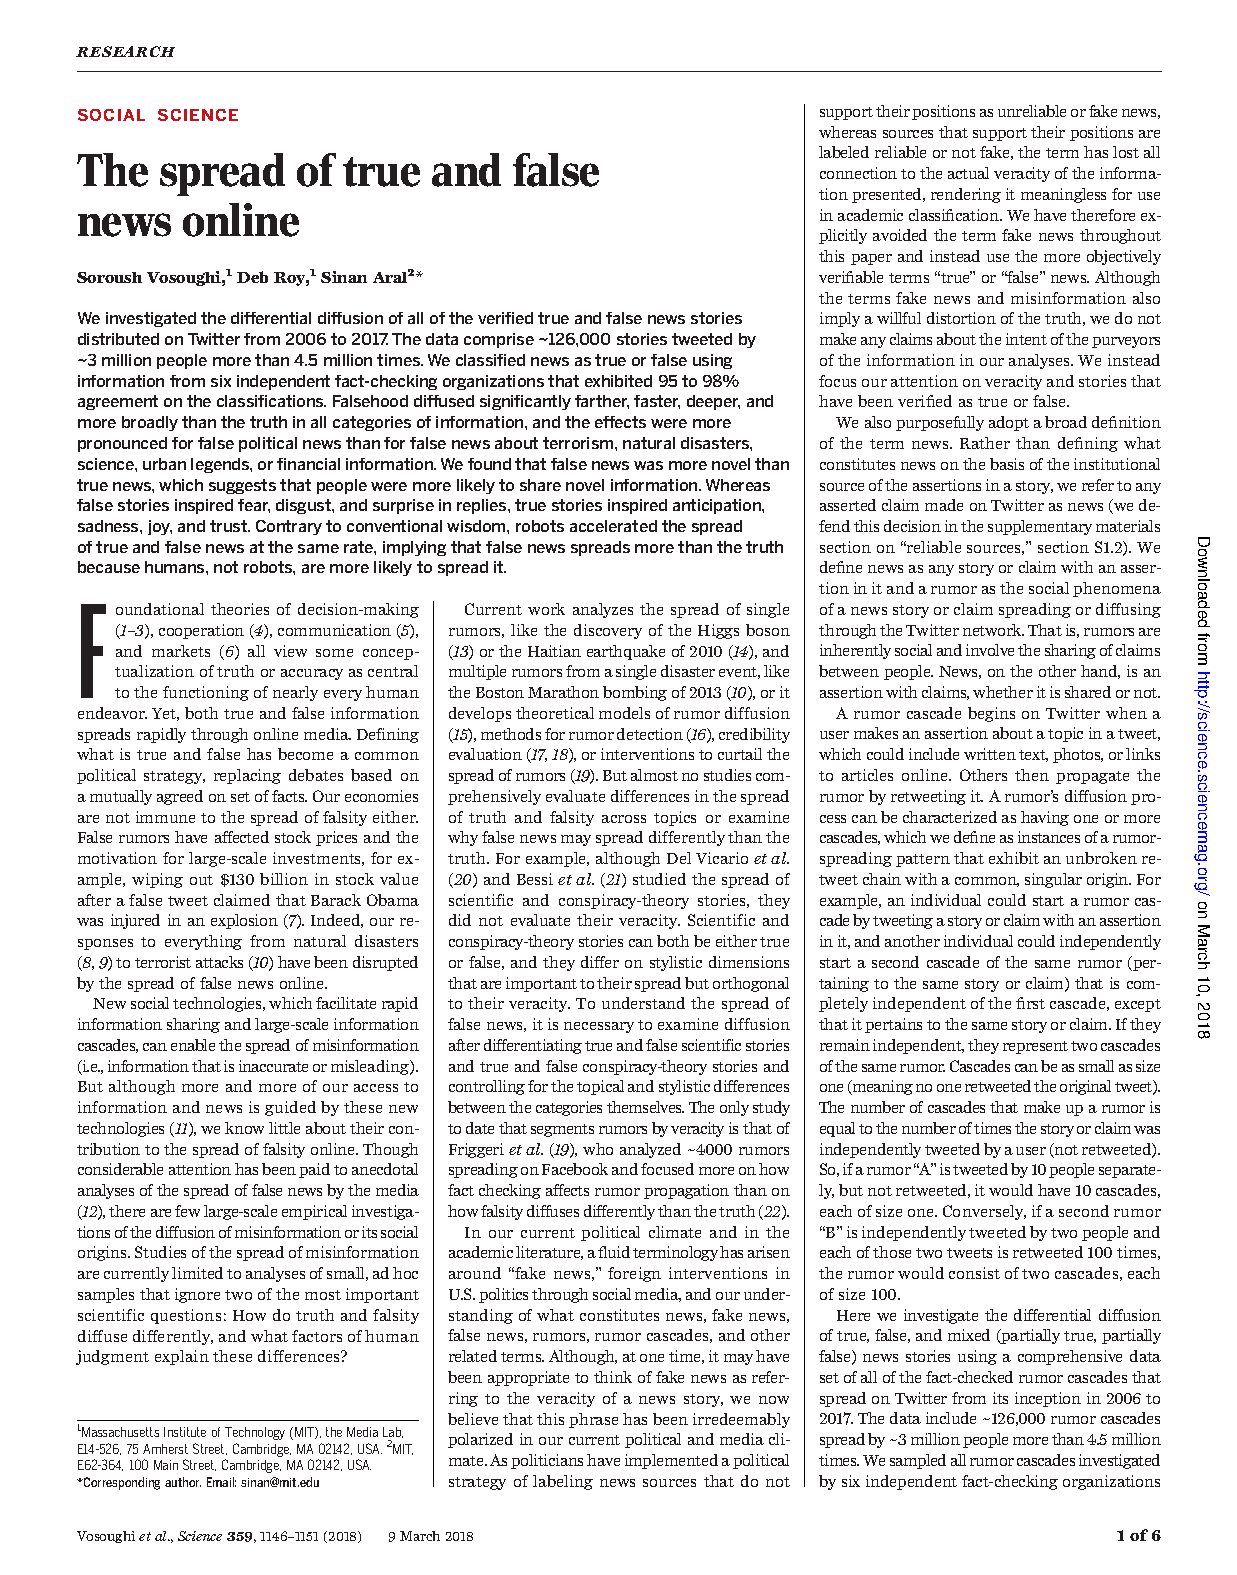
\includepdf[pages=1, scale=0.95, pagecommand=\heiti\sanhao{外\quad{}文\quad{}原\quad{}文}]{docs/translation.pdf}
% % 原文剩余部分
% \includepdf[pages=2-, scale=0.95, pagecommand={}]{docs/translation.pdf}
% \end{center}

% Translation
% \setcounter{chapter}{0}
% \renewcommand{\thefigure}{~外\arabic{chapter}-\arabic{figure}~}
% \renewcommand{\theequation}{~外\arabic{chapter}-\arabic{equation}~}
% \renewcommand{\thetable}{~外\arabic{chapter}-\arabic{table}~}

% \begin{center}
% \translationtitlefont{外\quad{}文\quad{}译\quad{}文}
% \end{center}
% \vspace{8mm}
% \thispagestyle{empty}


% \begin{center}
% \sanhao\heiti\textbf{真假新闻的在线传播}

% \xiaosihao\songti{Soroush Vosoughi, Deb Roy, Sinan Aral}

% \xiaosihao\songti{麻省理工学院}
% \end{center}

% \songti{}
% \begingroup % 限制两个let语句的作用范围在外文译文部分
% \let\clearpage\relax
% \let\cleardoublepage\relax

% %以下是排版示例,在这里为了使章节编号不出现在目录中,使用了无编号的样式,代价是这些数字都要自己书写。另外,由于外文文献一般不是很长,为了排版紧凑,每一章被设置为不另起一页。

% \chapter*{第一章\quad{}概述}
% %每一个chapter后记得以下两行
% \newtranschapter

% \section*{1.1\quad{}概述}
% 决策、合作、通信和市场领域的基础理论全都将对真实或准确度的概念化作为几乎一切人类努力的核心。然而,不论是真实信息还是虚假信息都会于在线媒体上迅速传播。定义什么是真、什么是假成了一种常见的政治策略,而不是基于一些各方同意的事实的争论。我们的经济也难免遭受虚假信息传播的影响。虚假流言会影响股价和大规模投资的动向,例如,在一条声称巴拉克·奥巴马在爆炸中受伤的推文发布后,股市市值蒸发了1300亿美元。的确,从自然灾害到恐怖袭击,我们对一切事情的反应都受到了扰乱。

% 新的社交网络技术在使信息的传播速度变快和规模变大的同时,也便利了不实信息(即不准确或有误导性的信息)的传播。然而,尽管我们对信息和新闻的获取越来越多地收到这些新技术的引导,但我们仍然对他们在虚假信息传播上的作用知之甚少。尽管媒体对假新闻传播的轶事分析给予了相当多的关注,但仍然几乎没有针对不实信息扩散或其发布源头的大规模实证调查。目前,虚假信息传播的研究仅仅局限于小的、局部的样本的分析上,而这些分析忽略了两个最重要的科学问题:真实信息和虚假信息的传播有什么不同?哪些人类判断中的因素可以解释这些不同?

% \begin{equation}
% \label{PCA_goal_appx1}
% \begin{aligned}
% \max_{\substack{\bm{W}}}  &  tr(\bm{W}^\mathrm{T}\bm{X}\bm{X}^ \mathrm{T}\bm{W})
% \end{aligned}
% \end{equation}

% 我只是为了把第二章挤到下一页而凑的字。我只是为了把第二章挤到下一页而凑的字。我只是为了把第二章挤到下一页而凑的字。我只是为了把第二章挤到下一页而凑的字。我只是为了把第二章挤到下一页而凑的字。我只是为了把第二章挤到下一页而凑的字。我只是为了把第二章挤到下一页而凑的字。我只是为了把第二章挤到下一页而凑的字。我只是为了把第二章挤到下一页而凑的字。我只是为了把第二章挤到下一页而凑的字。我只是为了把第二章挤到下一页而凑的字。我只是为了把第二章挤到下一页而凑的字。我只是为了把第二章挤到下一页而凑的字。我只是为了把第二章挤到下一页而凑的字。我只是为了把第二章挤到下一页而凑的字。我只是为了把第二章挤到下一页而凑的字。我只是为了把第二章挤到下一页而凑的字。我只是为了把第二章挤到下一页而凑的字。我只是为了把第二章挤到下一页而凑的字。我只是为了把第二章挤到下一页而凑的字。我只是为了把第二章挤到下一页而凑的字。我只是为了把第二章挤到下一页而凑的字。我只是为了把第二章挤到下一页而凑的字。我只是为了把第二章挤到下一页而凑的字。

% \chapter*{第二章\quad{}我也不知道是什么}
% \newtranschapter

% 新的社交网络技术在使信息的传播速度变快和规模变大的同时,也便利了不实信息(即不准确或有误导性的信息)的传播。然而,尽管我们对信息和新闻的获取越来越多地收到这些新技术的引导,但我们仍然对他们在虚假信息传播上的作用知之甚少。尽管媒体对假新闻传播的轶事分析给予了相当多的关注,但仍然几乎没有针对不实信息扩散或其发布源头的大规模实证调查。目前,虚假信息传播的研究仅仅局限于小的、局部的样本的分析上,而这些分析忽略了两个最重要的科学问题:真实信息和虚假信息的传播有什么不同?哪些人类判断中的因素可以解释这些不同?

% 新的社交网络技术在使信息的传播速度变快和规模变大的同时,也便利了不实信息(即不准确或有误导性的信息)的传播。然而,尽管我们对信息和新闻的获取越来越多地收到这些新技术的引导,但我们仍然对他们在虚假信息传播上的作用知之甚少。尽管媒体对假新闻传播的轶事分析给予了相当多的关注,但仍然几乎没有针对不实信息扩散或其发布源头的大规模实证调查。目前,虚假信息传播的研究仅仅局限于小的、局部的样本的分析上,而这些分析忽略了两个最重要的科学问题:真实信息和虚假信息的传播有什么不同?哪些人类判断中的因素可以解释这些不同?

% 新的社交网络技术在使信息的传播速度变快和规模变大的同时,也便利了不实信息(即不准确或有误导性的信息)的传播。然而,尽管我们对信息和新闻的获取越来越多地收到这些新技术的引导,但我们仍然对他们在虚假信息传播上的作用知之甚少。尽管媒体对假新闻传播的轶事分析给予了相当多的关注,但仍然几乎没有针对不实信息扩散或其发布源头的大规模实证调查。目前,虚假信息传播的研究仅仅局限于小的、局部的样本的分析上,而这些分析忽略了两个最重要的科学问题:真实信息和虚假信息的传播有什么不同?哪些人类判断中的因素可以解释这些不同?

% \begin{equation}
% \label{PCA_goal_appx2}
% \begin{aligned}
% \max_{\substack{\bm{W}}}  &  tr(\bm{W}^\mathrm{T}\bm{X}\bm{X}^ \mathrm{T}\bm{W})
% \end{aligned}
% \end{equation}

% 新的社交网络技术在使信息的传播速度变快和规模变大的同时,也便利了不实信息(即不准确或有误导性的信息)的传播。然而,尽管我们对信息和新闻的获取越来越多地收到这些新技术的引导,但我们仍然对他们在虚假信息传播上的作用知之甚少。尽管媒体对假新闻传播的轶事分析给予了相当多的关注,但仍然几乎没有针对不实信息扩散或其发布源头的大规模实证调查。目前,虚假信息传播的研究仅仅局限于小的、局部的样本的分析上,而这些分析忽略了两个最重要的科学问题:真实信息和虚假信息的传播有什么不同?哪些人类判断中的因素可以解释这些不同?

% 新的社交网络技术在使信息的传播速度变快和规模变大的同时,也便利了不实信息(即不准确或有误导性的信息)的传播。然而,尽管我们对信息和新闻的获取越来越多地收到这些新技术的引导,但我们仍然对他们在虚假信息传播上的作用知之甚少。尽管媒体对假新闻传播的轶事分析给予了相当多的关注,但仍然几乎没有针对不实信息扩散或其发布源头的大规模实证调查。目前,虚假信息传播的研究仅仅局限于小的、局部的样本的分析上,而这些分析忽略了两个最重要的科学问题:真实信息和虚假信息的传播有什么不同?哪些人类判断中的因素可以解释这些不同?

% 新的社交网络技术在使信息的传播速度变快和规模变大的同时,也便利了不实信息(即不准确或有误导性的信息)的传播。然而,尽管我们对信息和新闻的获取越来越多地收到这些新技术的引导,但我们仍然对他们在虚假信息传播上的作用知之甚少。尽管媒体对假新闻传播的轶事分析给予了相当多的关注,但仍然几乎没有针对不实信息扩散或其发布源头的大规模实证调查。目前,虚假信息传播的研究仅仅局限于小的、局部的样本的分析上,而这些分析忽略了两个最重要的科学问题:真实信息和虚假信息的传播有什么不同?哪些人类判断中的因素可以解释这些不同?

% \endgroup

% 开题报告
% \blankmatter
% 
\includepdf[pages=-]{docs/openingReport.pdf}


% 中期检查表
% \blankmatter
% 
\includepdf[pages=-]{docs/interimReport.pdf}


\end{document}
